\chapter[System Description]{System Description}
\label{chap:descricaoproblema}


\section{EHDA}
\label{sec:ehda_resume}

\begin{figure}[H]
  \centering
  \resizebox{150mm}{!}{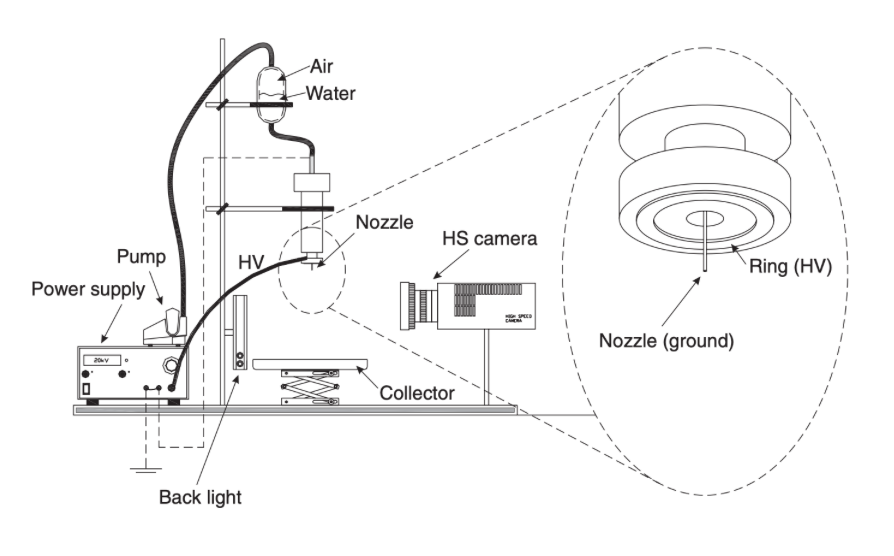
\includegraphics{Figuras/system_setup.png}}
  \caption{EHDA automation system setup}
  \label{fig:ehda_setup}
\end{figure}


\begin{figure}[H]
  \centering
  \resizebox{150mm}{!}{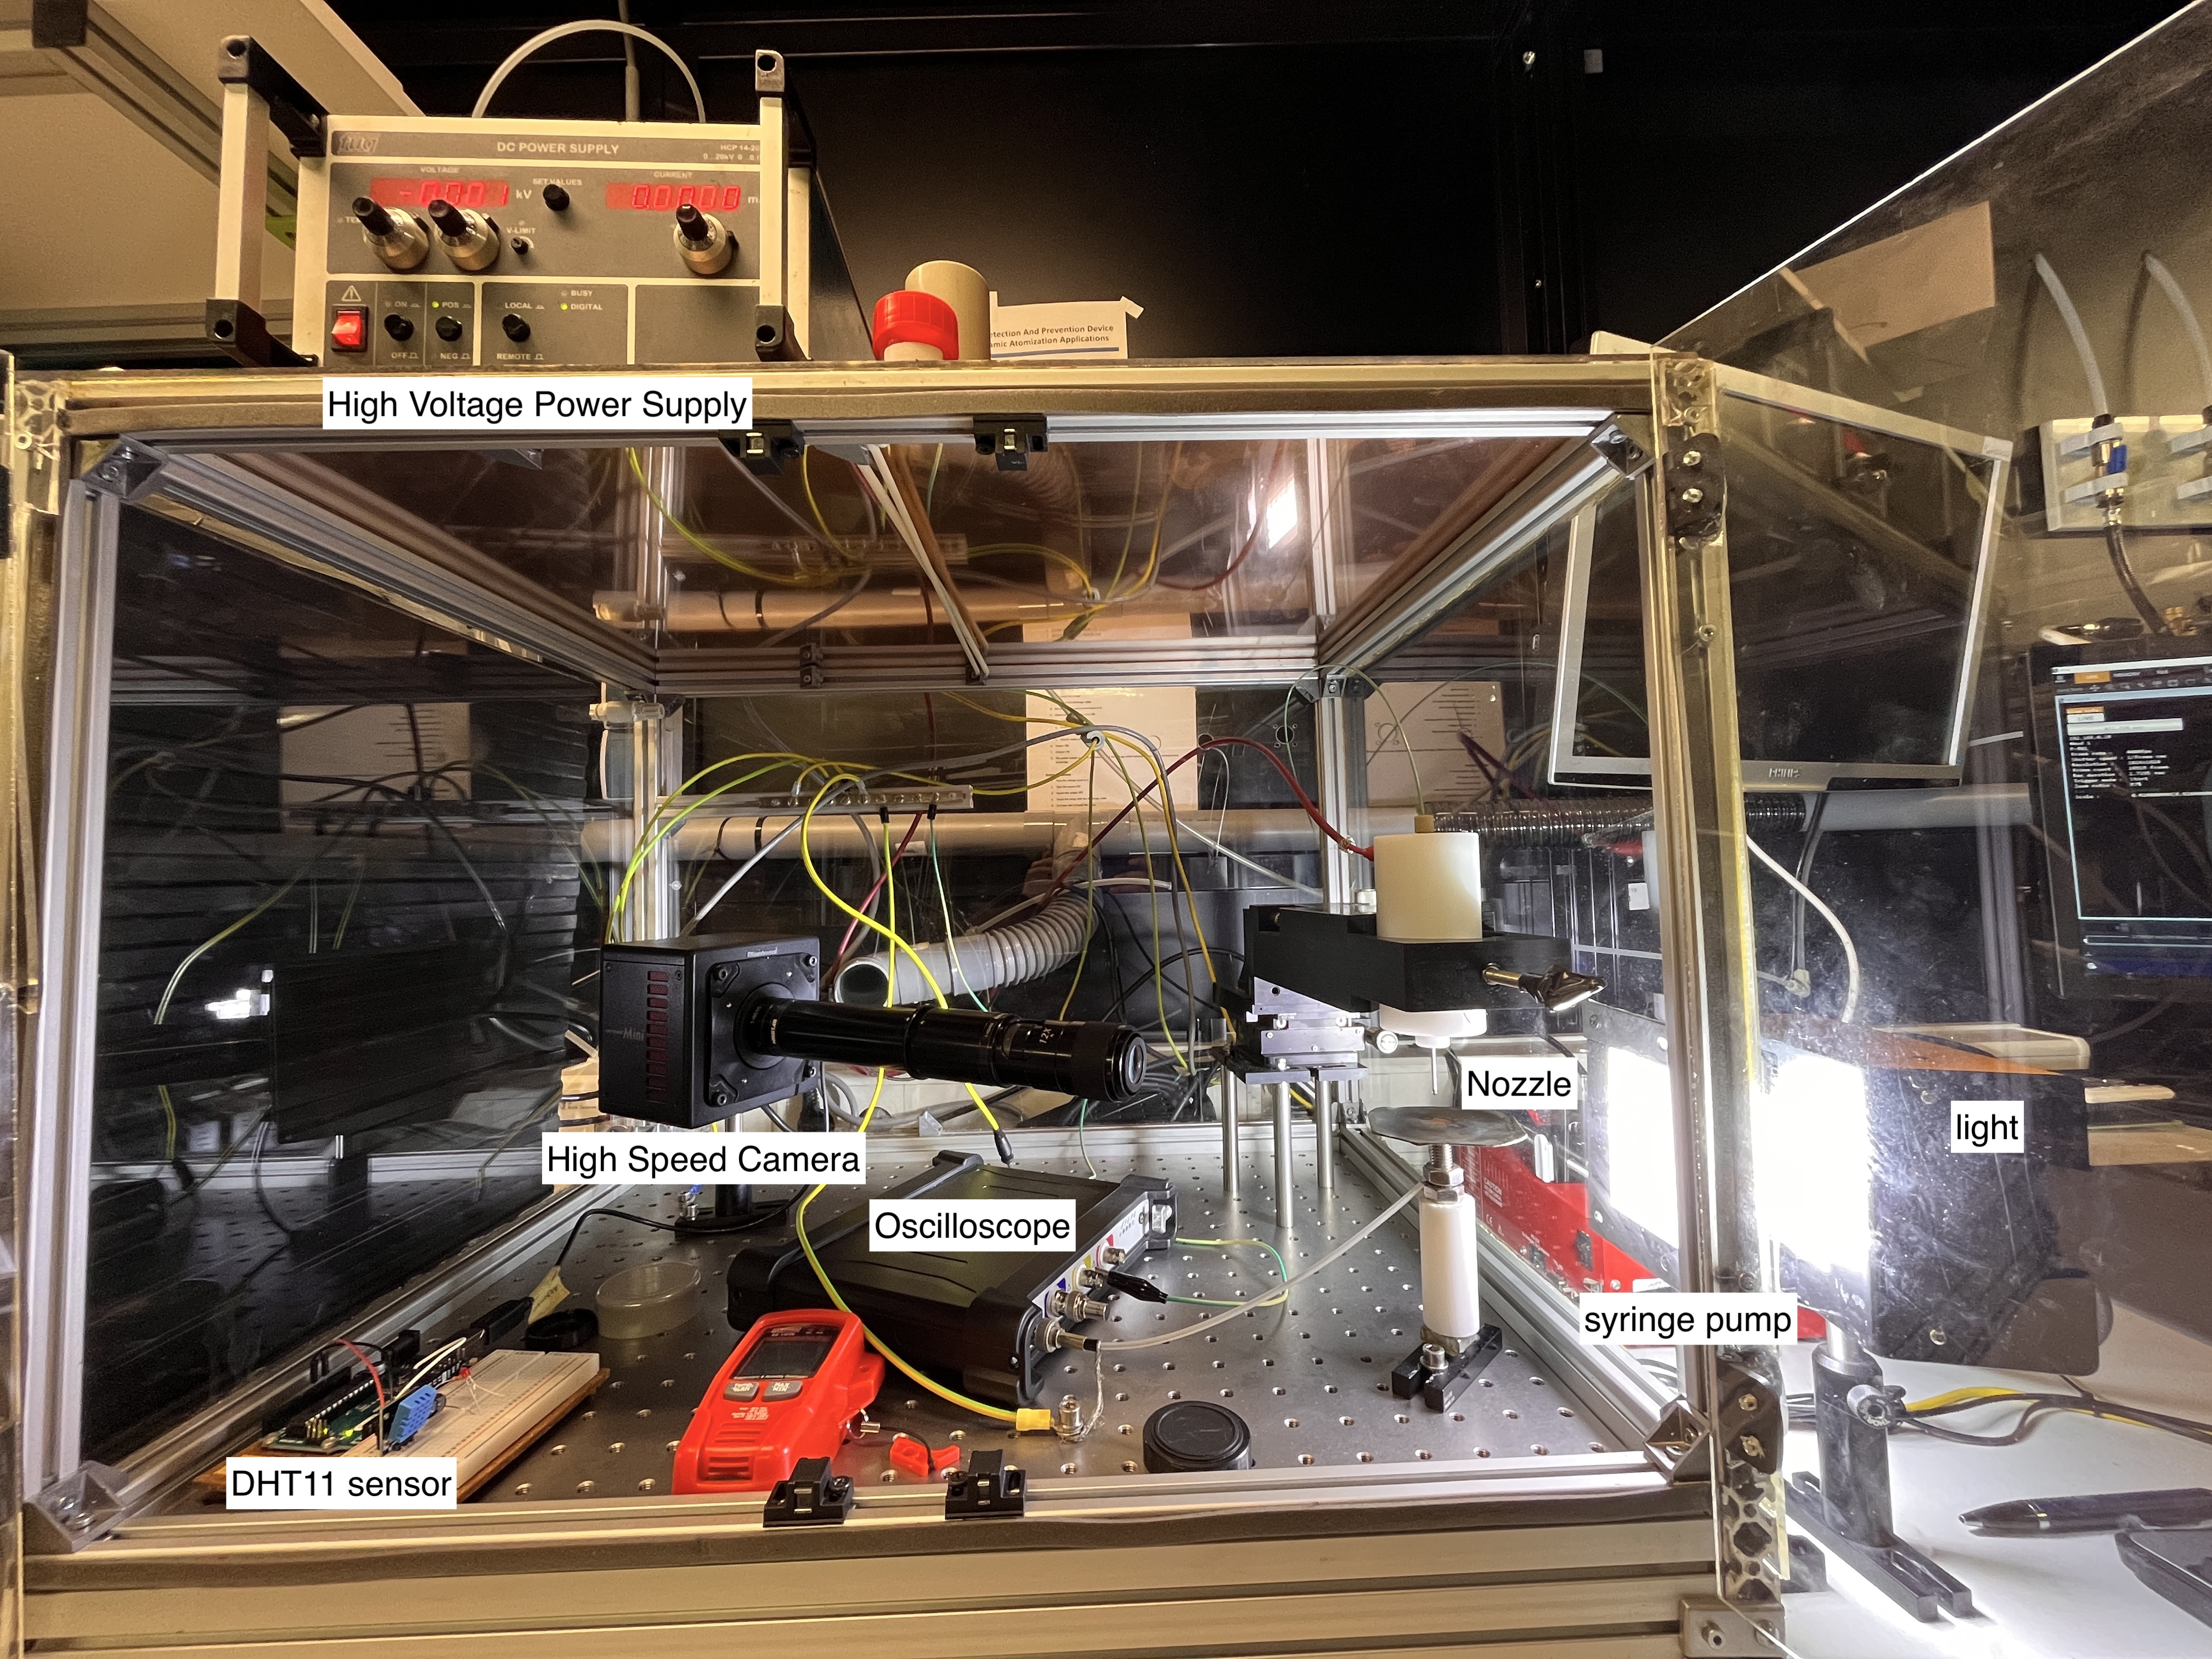
\includegraphics{Figuras/setup_pic.jpg}}
  \caption{EHDA automation system setup}
  \label{fig:setup_pic}
\end{figure}

\begin{multicols}{3}

  \begin{figure}[H]
      \center
      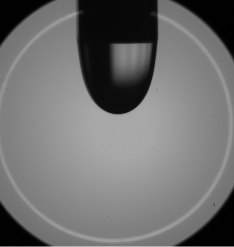
\includegraphics[width=3cm]{Figuras/drippingexample.png}
      \caption{Dripping}
  \end{figure}


  \begin{figure}[H]
      \center
      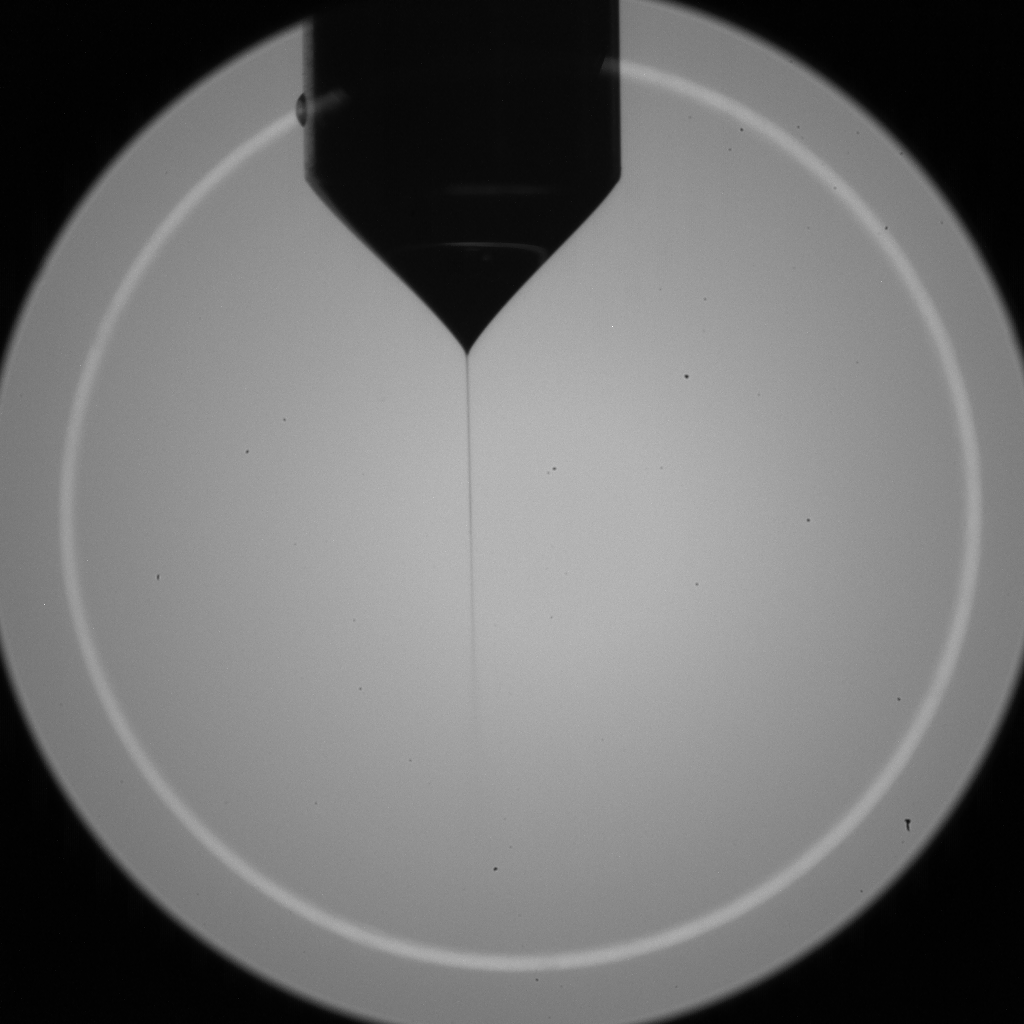
\includegraphics[width=3cm]{Figuras/conejetexample.png}
      \caption{Cone Jet}
  \end{figure}


  \begin{figure}[H]
      \center
      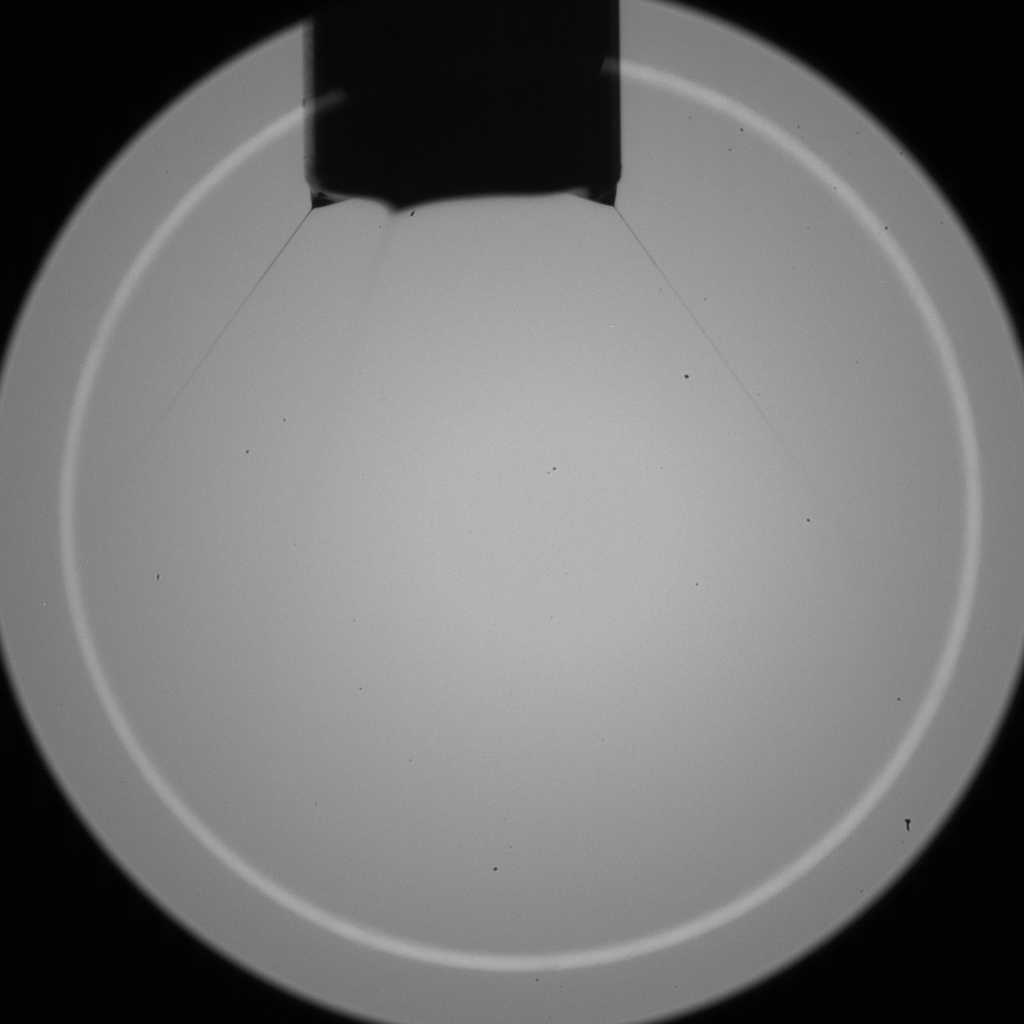
\includegraphics[width=3cm]{Figuras/multijetexample.png}
      \caption{Multi Jet}
  \end{figure}

\end{multicols}




\section{Instrumentation}
\label{sec:instrumentation}

The peripherals automation routine was already developed by another student. In order to continue the research I took some time to understand the physical concept behind EHDA experiments and the project knowledge.
I made upgrades in the routine to include the high speed camera with a hardware triggering routine using an arduino microcontroler. This will be usefull to validate the further classification of the spray dynamics.


% ilustramos o processo com a Figura \ref{fig:setup}. 

\begin{figure}[H]
  \centering
  \resizebox{150mm}{!}{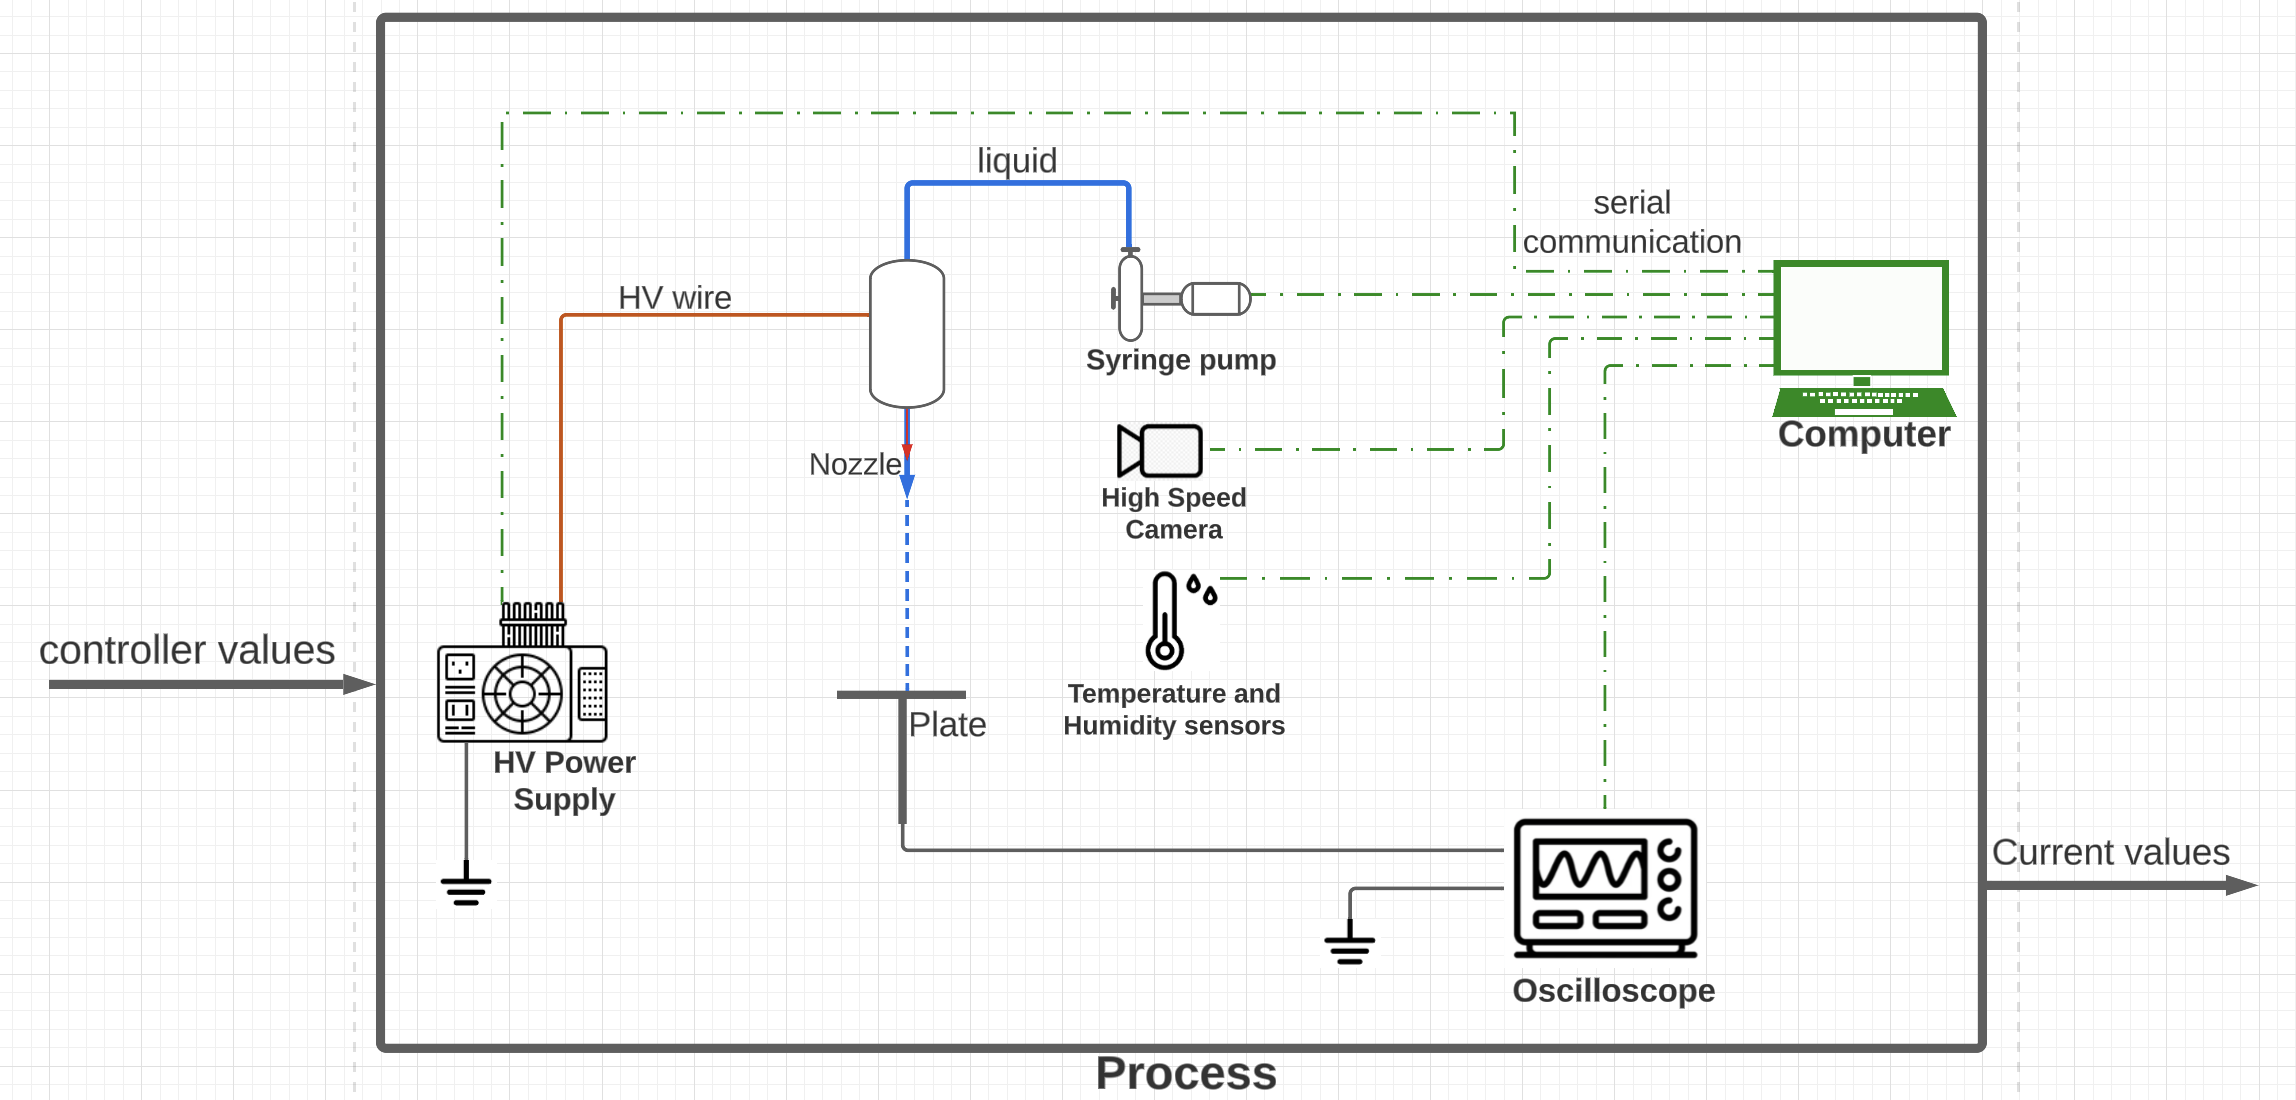
\includegraphics{Figuras/new_system_setup.png}}
  \caption{EHDA automation system setup}
  \label{fig:setup}
\end{figure}


\section{First Experiments}
\label{sec:first_experiments}

Initial tests were made to verify the setup assembly and the automation routine integration. In this step I could unterstand in practise how electrospray works.
I noticed that we need a large set of variables in the range to produce the desired dynamics of electrospray, which most of the time is cone-jet mode. Those variables can be the liquid properties such as surface tension, dielectric constant, viscosity, density, electrical conductivity and vacuum permitivity. And also physical variables such as flowrate, system impedance, system temperature, system humidity, nozzle to plate distance, nozzle dimensions and applied voltage.
The instruments used in the setup are:

\begin{enumerate}[a]
  \item High Voltage Power Supply (FUG)
  \item Oscilloscope TiePie WS6 DIFF 
  \item Humidity and Temperature sensor (DHT11 + Arduino Uno)
  \item High Speed Camera - Photron fastcam mini
  \item Syringe pump
  \end{enumerate}

\begin{figure}[H]
  \centering
  \resizebox{150mm}{!}{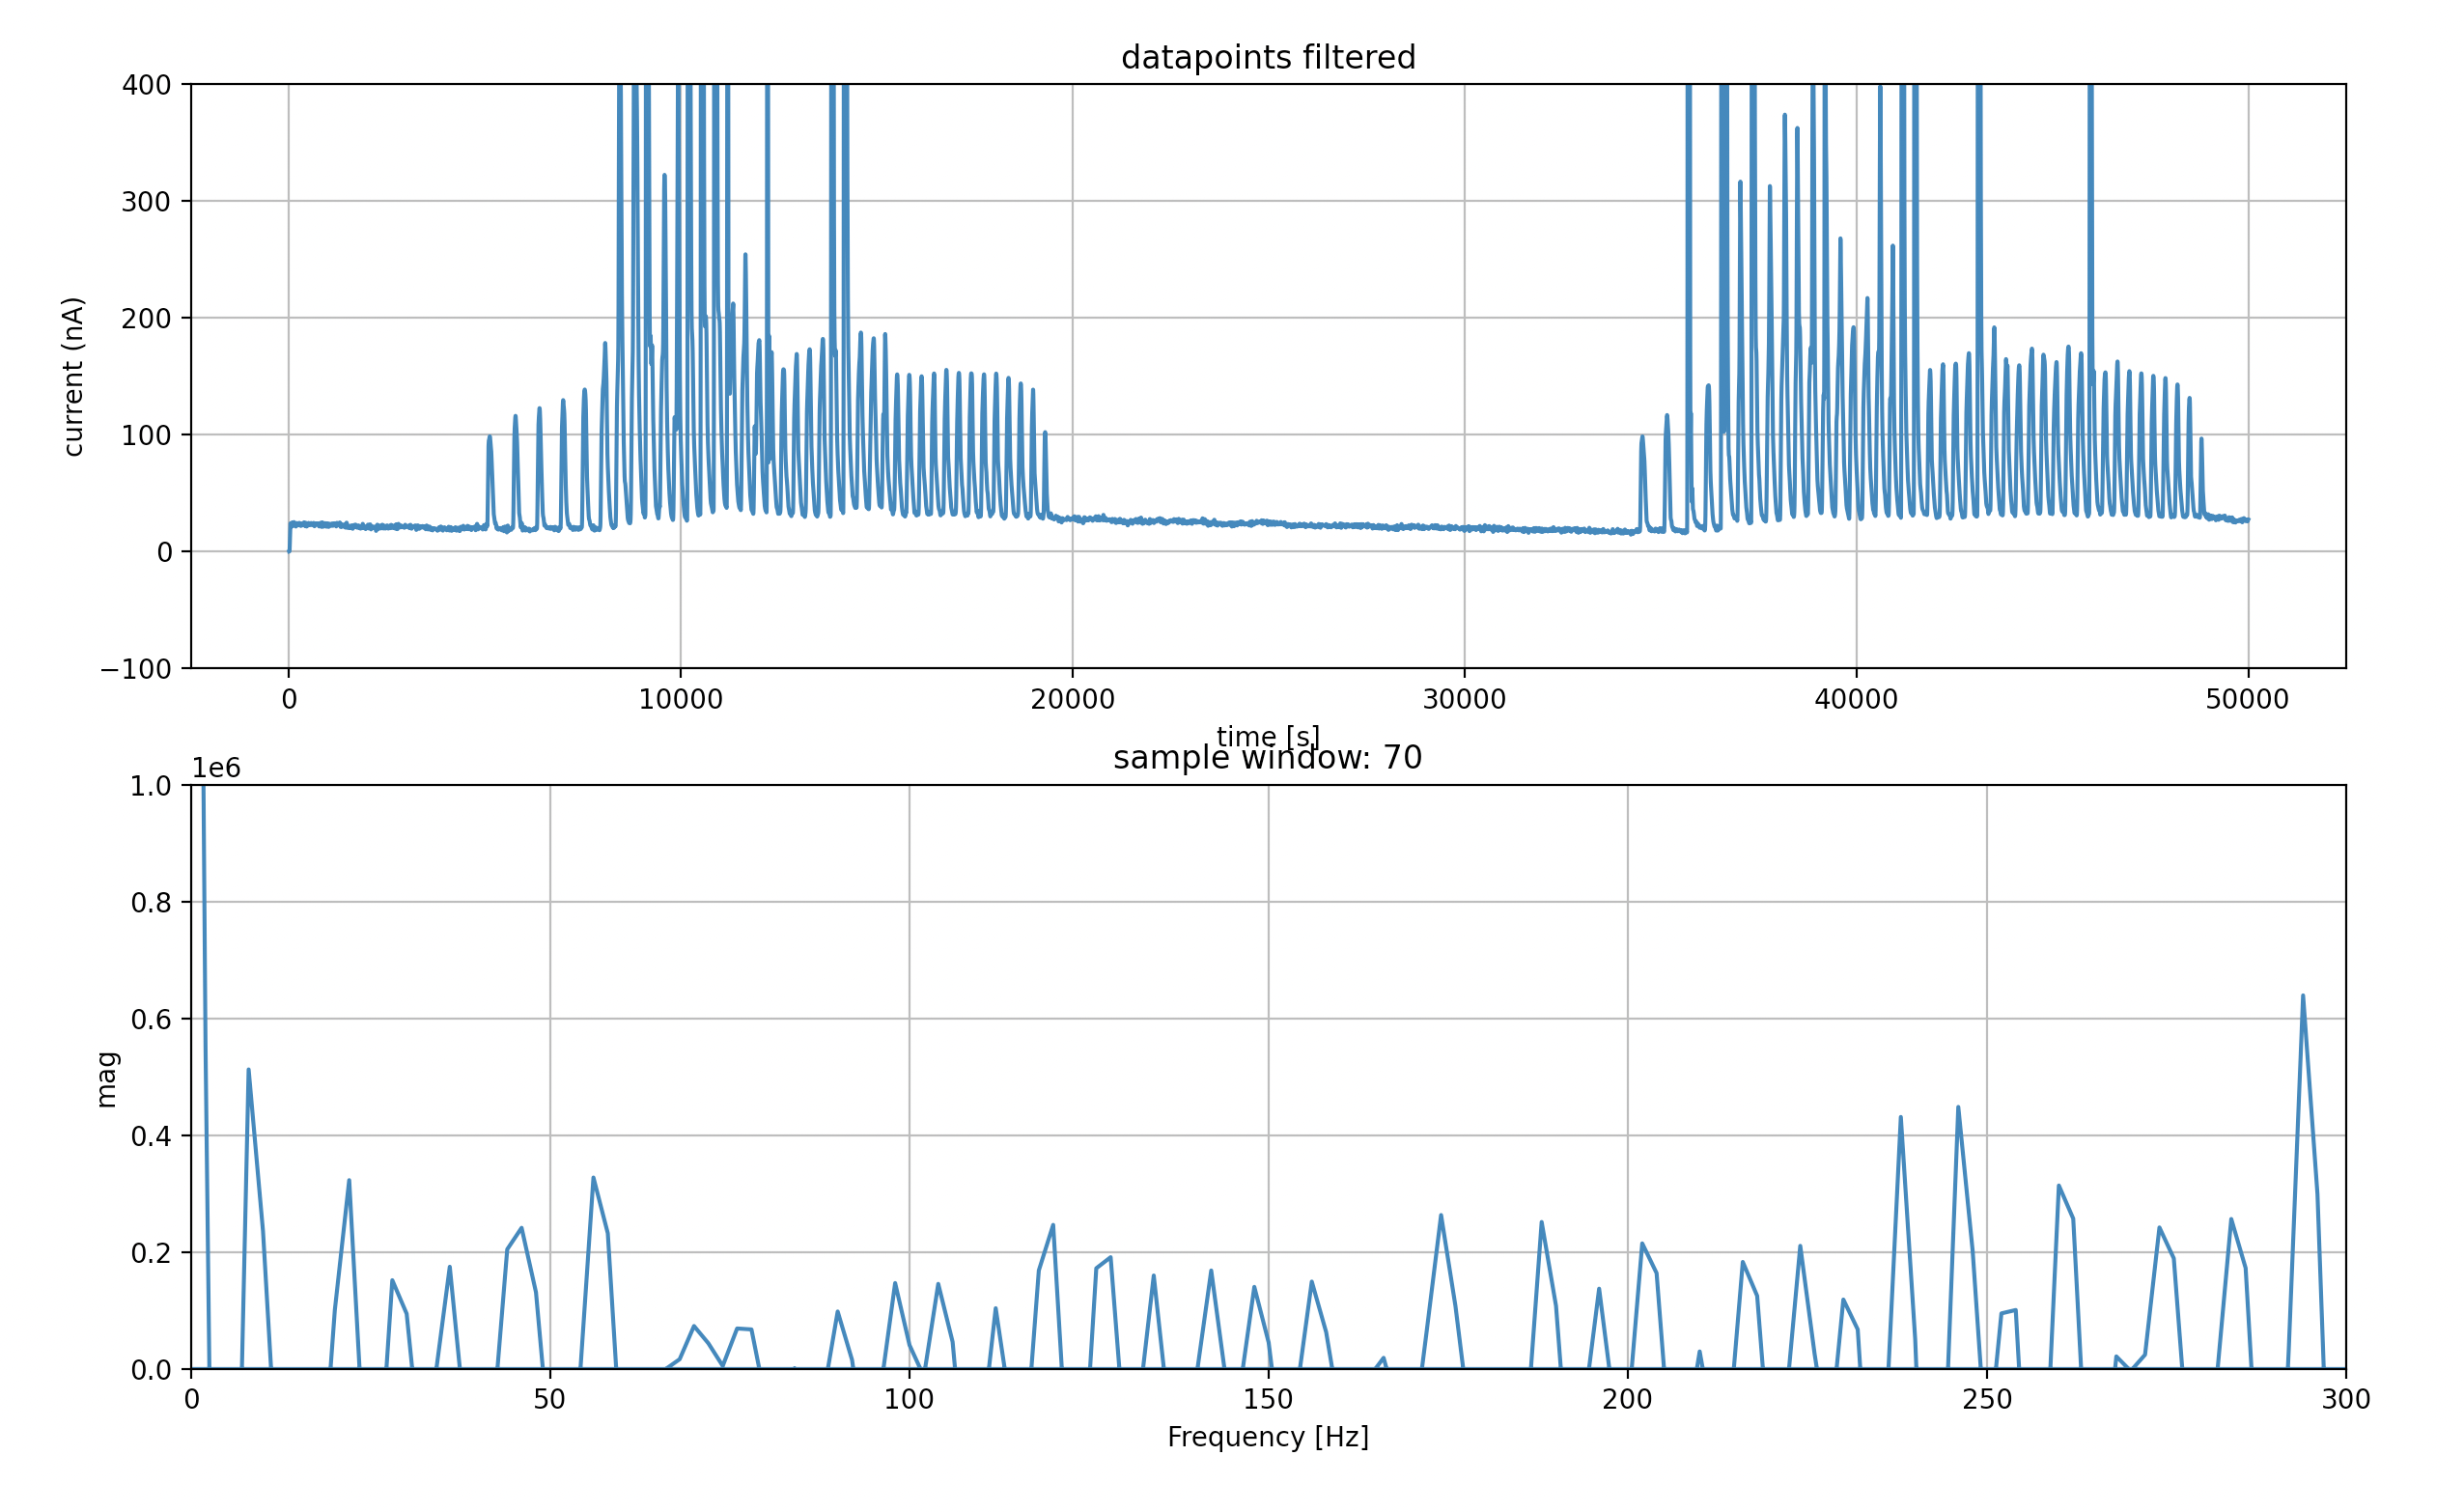
\includegraphics{Figuras/report2/img2.png}}
  \caption{EHDA automation system setup}
  \label{fig:microdripping_current_pic}
\end{figure}

\clearpage
